%%%%%%%%%%%%%%%%%%%%%%%%%%%%%%%%%%%%

\section{実験}

%%%%%%%%%%%%%%%%%%%%%%%%%%%%%%%%%%%%

\begin{frame}
\frametitle{実験計画の原則}

\begin{enumerate}

\item \hl{統制：}直接研究している変数以外の変数の（潜在的な）影響を統制する。

\item \hl{無作為化：}可能な限り、被験者を処置にランダムに割り当て、
母集団からランダムにサンプリングする。

\item \hl{反復：}研究内では十分に大きな標本を収集することで反復する。
あるいは研究全体を繰り返す。

\item \hl{ブロッキング：}応答変数に影響を与えることが分かっている、
または疑われる変数がある場合、まずその変数に基づいて被験者を
\hl{ブロック}にグループ化し、各ブロック内でケースを処置群にランダムに割り当てる。

\end{enumerate}

\end{frame}

%%%%%%%%%%%%%%%%%%%%%%%%%%%%%%%%%%%%

\begin{frame}
\frametitle{ブロッキングについて詳しく}

\twocol{0.25}{0.75}
{
\begin{center}

\includegraphics[width=\textwidth]{1-4_experiments/figures/gu}
\end{center}
}
{
\begin{itemize}
\item エナジーゲルが走力を向上させるかを調べる実験を設計したい：

\begin{itemize}
\item 処置群：エナジーゲルあり
\item 対照群：エナジーゲルなし
\end{itemize}

\item エナジーゲルがプロとアマチュアのアスリートに異なる影響を与えると疑われるため、
プロかどうかでブロッキングを行う：

\begin{itemize}
\item 標本をプロとアマチュアに分ける
\item プロのアスリートを処置群と対照群にランダムに割り当てる
\item アマチュアのアスリートを処置群と対照群にランダムに割り当てる
\item これにより、処置群と対照群にプロ・アマチュアが均等に代表される
\end{itemize}
\end{itemize}
}

\dq{なぜこれが重要か？ 他にブロッキングすべき変数はあるか？}

\end{frame}

%%%%%%%%%%%%%%%%%%%%%%%%%%%%%%%%%%%%

\begin{frame}
\frametitle{練習問題}

\pq{照明レベルと騒音レベルが学生の試験成績に与える影響を調べる研究を設計する。
研究者は照明と騒音が男女で異なる効果を持つ可能性があると考え、
両性が各グループに均等に含まれるようにしたいと考えている。
次のうち正しいものはどれか？}

\begin{enumerate}[(a)]
\item 説明変数が3つ（照明・騒音・性別）、応答変数が1つ（試験成績）である。
\solnMult{説明変数が2つ（照明と騒音）、ブロッキング変数が1つ（性別）、応答変数が1つ（試験成績）である。}
\item 説明変数が1つ（性別）、応答変数が3つ（照明・騒音・試験成績）である。
\item ブロッキング変数が2つ（照明と騒音）、説明変数が1つ（性別）、応答変数が1つ（試験成績）である。
\end{enumerate}

\end{frame}

%%%%%%%%%%%%%%%%%%%%%%%%%%%%%%%%%%%%

\begin{frame}
\frametitle{ブロッキング変数と説明変数の違い}

\begin{itemize}

\item 要因（factor）とは、実験単位に課すことができる条件のことである。

\item ブロッキング変数とは、実験単位がもともと持っている特性であり、
その影響を統制したいものである。

\item ブロッキングは層化に似ているが、
サンプリングの際ではなく実験設定においてランダムに割り当てる際に用いられる。

\end{itemize}

\end{frame}

%%%%%%%%%%%%%%%%%%%%%%%%%%%%%%%%%%%%

\begin{frame}
\frametitle{実験計画の用語（続き）}

\begin{itemize}

\item \hl{プラセボ：}偽の処置。医学研究では対照群に用いられることが多い。

\item \hl{プラセボ効果：}特別な処置を受けていると信じるだけで、
実験単位が改善を示す現象。

\item \hl{盲検化（ブラインディング）：}実験単位が自分が対照群か処置群かを
知らない状態にすること。

\item \hl{二重盲検：}実験単位と、患者に関わる研究者の両方が、
誰が対照群で誰が処置群かを知らない状態にすること。

\end{itemize}

\end{frame}

%%%%%%%%%%%%%%%%%%%%%%%%%%%%%%%%%%%%

\begin{frame}
\frametitle{練習問題}

\pq{観察研究と実験の主な違いは何か？}

\begin{enumerate}[(a)]
\item 実験は研究室で行われるが、観察研究は必ずしも研究室で行う必要はない。
\item 観察研究では過去に起きたことしか調べられない。
\solnMult{ほとんどの実験では無作為割り当てを用いるが、観察研究では用いない。}
\item 観察研究は、その結果から因果推論ができないため、まったく役に立たない。
\end{enumerate}

\end{frame}

%%%%%%%%%%%%%%%%%%%%%%%%%%%%%%%%%%%%

\begin{frame}
\frametitle{無作為割り当てと無作為抽出}

\begin{center}
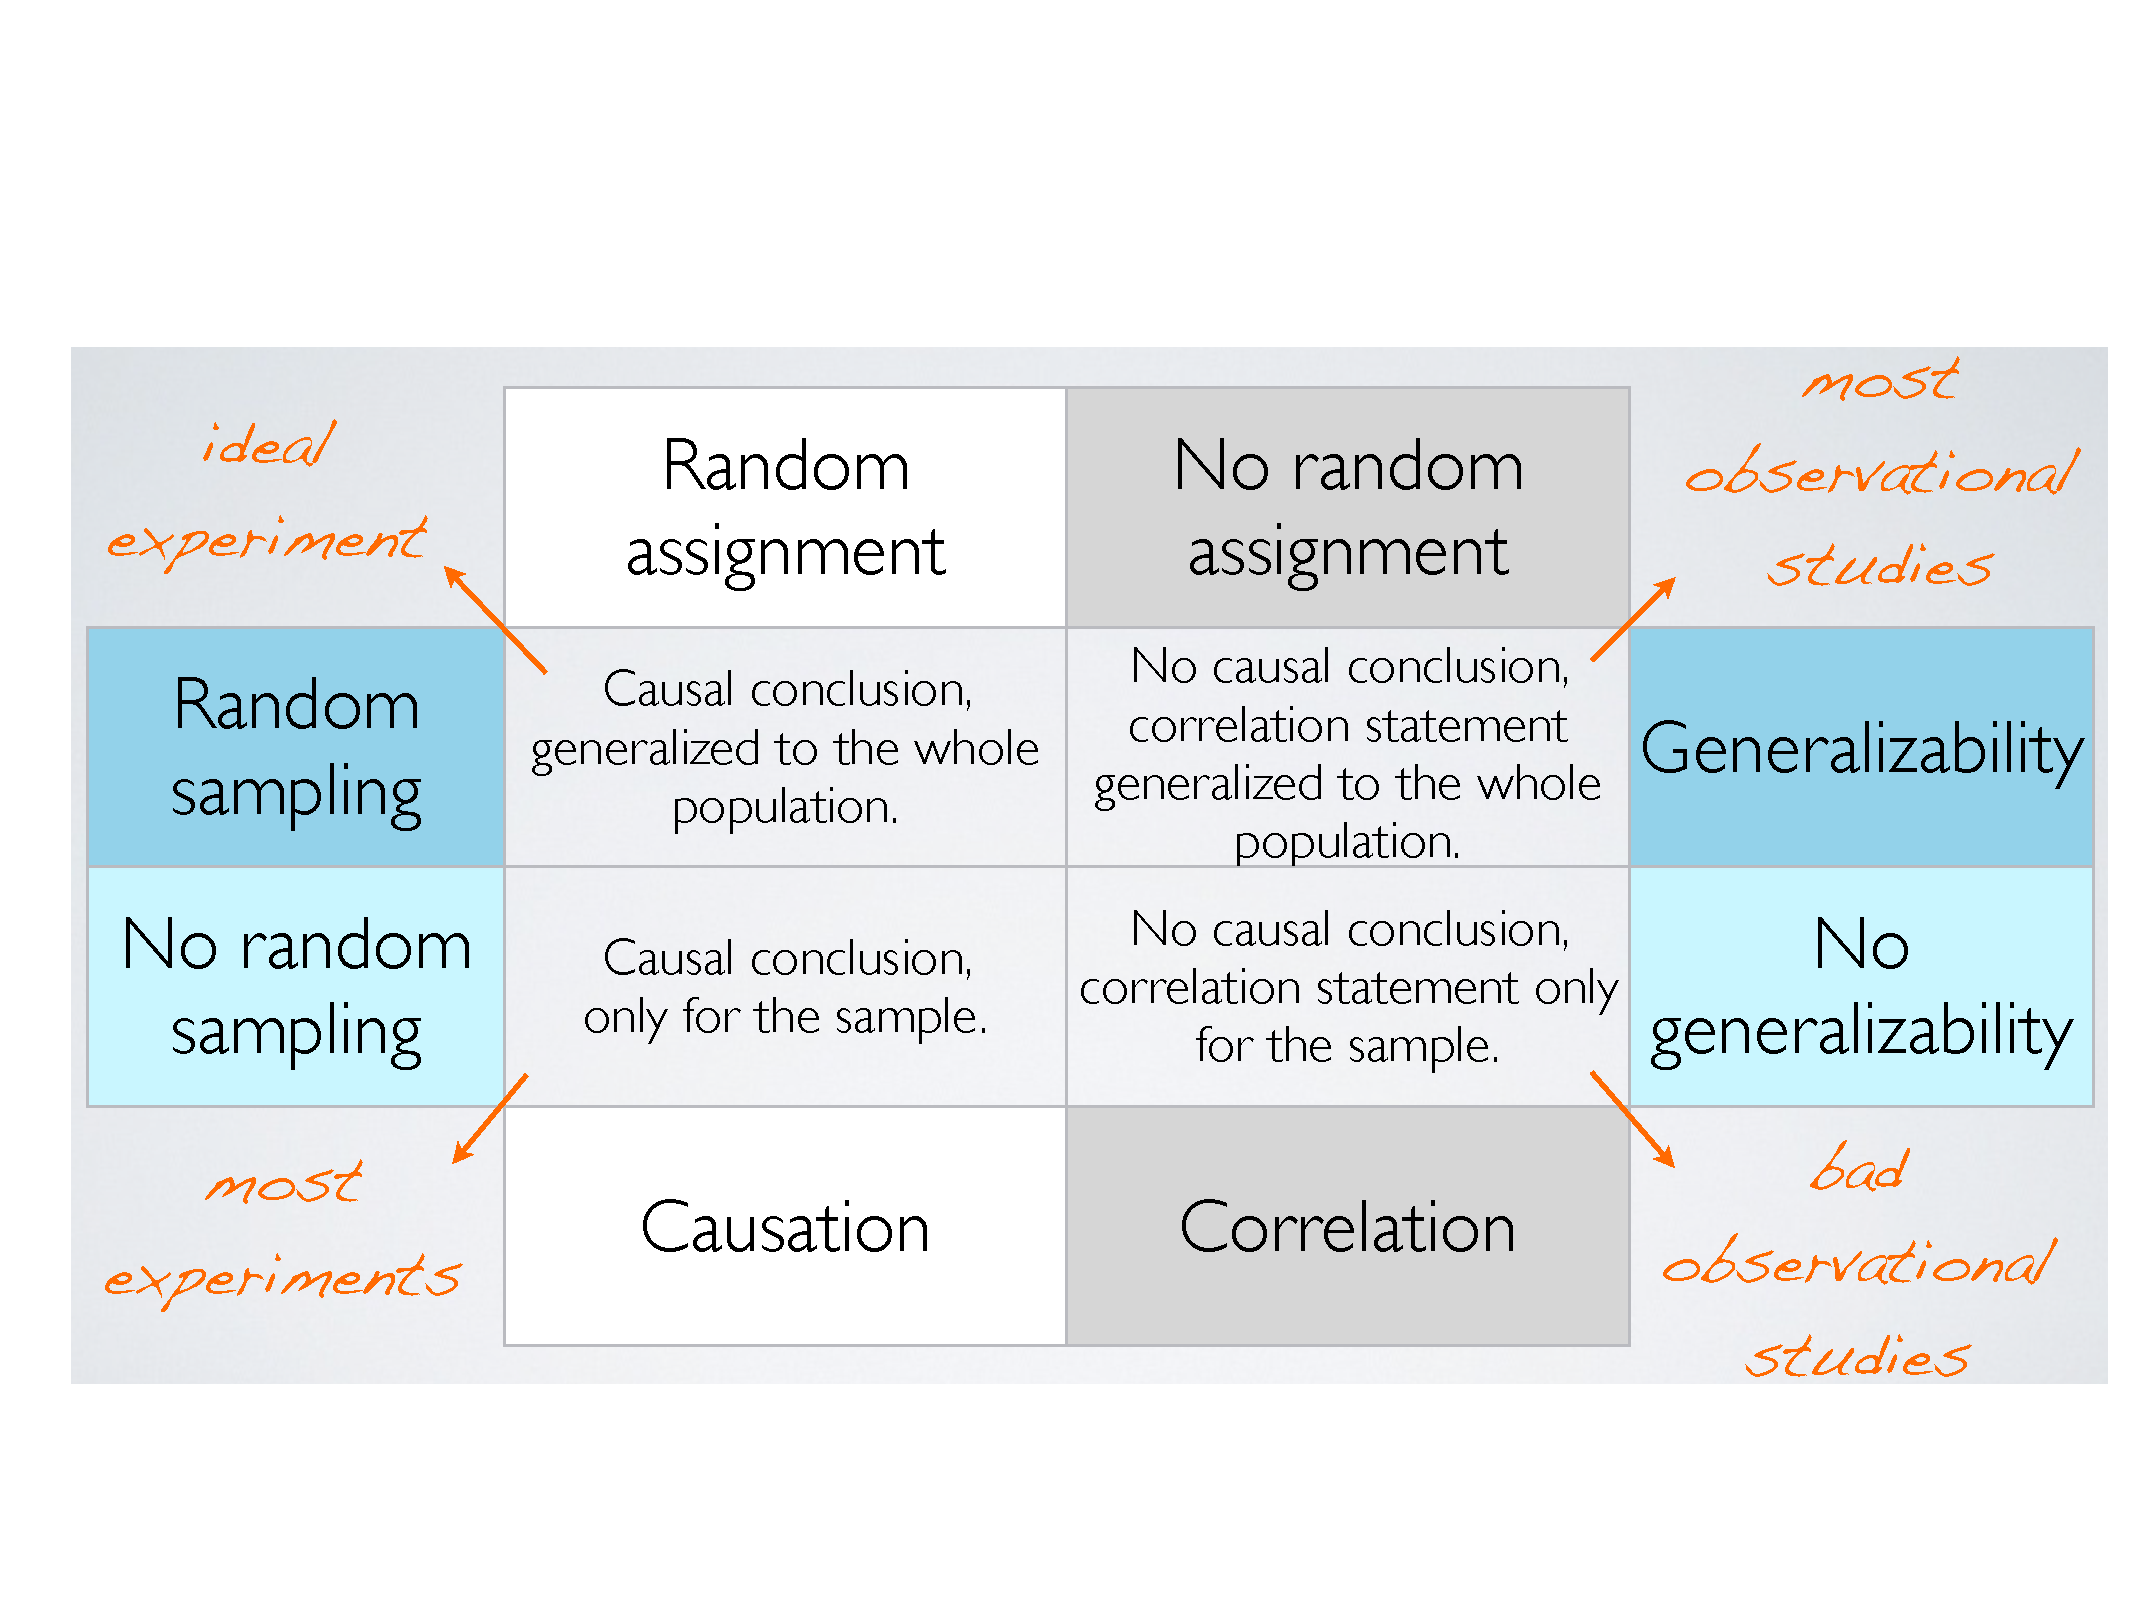
\includegraphics[width=\textwidth]{1-4_experiments/figures/random_sample_assignment}
\end{center}

\end{frame}

%%%%%%%%%%%%%%%%%%%%%%%%%%%%%%%%%%%%
